\chapter{Preliminaries: Dynamical Systems. and Topology}

This chapter provides a self-contained introduction to several mathematical frameworks—dynamical systems, topology and logical type theory -- that serve as conceptual reference points for the formalism developed in subsequent chapters. 

Dynamic systems theory is important as it's our way of operationally and phenomenologically understanding generative meaning and intelligence. Topology is important as its structural motifs and representational strategies are core to Homotopy Type Theory. And type theoretic preliminaries set the scene for the core calculus of our logic of meaning. 

These areas are generally distinct and unrelated disciplines. Our engagement with these areas is interpretive, generative and symboiotic: we employ their rich vocabularies within the topology of matehamtical disciplines to adapt and reconfigure and yield what will become a logic of this very process of mathematical play as an exemplar -- Dynamic Homotopy Type Theory (DHoTT).

The aim here is not to rehearse disciplinary detail, but to equip the reader with a shared conceptual foundation—a common semantic landscape—from which our more novel constructions can unfold. For some readers, this material may serve as a useful review; for others, it may be a first encounter. In either case, our intention is to establish a sufficiently coherent background that allows the reader to situate the ensuing formal development with clarity.

Importantly, this chapter is not required reading in a strict sense. Readers already familiar with the mathematical language of flows, fields, and manifolds may skim or skip it without disruption. The core theoretical machinery begins in earnest with Chapter 3. However, for those interested in the deeper conceptual resonances between our formalism and the classical mathematical disciplines from which it draws, this chapter may serve as a valuable orienting framework.

\section{Dynamical Systems}

%--------------------------------------------------
% Motivation + Definition of a Dynamical System
%--------------------------------------------------

\subsection{Flows and trajectories}

Before formalising the concept, recall the intuition:

\begin{itemize}
  \item \textbf{State $\to$ trajectory.}  Physical, biological, and computational
        processes are rarely static; they \emph{move}.  A dynamical system
        captures that motion by assigning to each initial condition a
        \emph{trajectory} through state space.
  \item \textbf{Time as a parameter.}  Whether time is measured in
        continuous seconds ($\mathbb R$) or discrete clock ticks
        ($\mathbb Z$), we want a single framework that treats both cases
        uniformly.
  \item \textbf{Deterministic rule.}  Once the present state is known,
        the future (and the past) are fixed by a deterministic \emph{flow}
        map~$\phi$.\footnote{Stochastic generalisations replace
        determinism by probability kernels; see, e.g.\ Markov processes.}
  \item \textbf{Composition in time.}  The whole purpose is to predict
        \emph{long-run} behaviour, so advancing by~$t+s$ must coincide
        with advancing first by~$s$ and then by~$t$.
\end{itemize}

These four ideas crystallise into the following definition.

\begin{definition}[Dynamical System]
A \emph{dynamical system} is a triple $(X, T, \phi)$, where:
\begin{itemize}
  \item $X$ is a set, called the \emph{state space}.
  \item $T$ is the \emph{time domain}, typically $\mathbb{R}$
        (continuous time) or $\mathbb{Z}$ (discrete time).
  \item $\phi : T \times X \to X$ is a map, called the \emph{flow},
        satisfying:
    \begin{enumerate}
      \item (identity) $\phi(0, x) = x$ for all $x \in X$;
      \item (composition) $\phi(t+s, x) = \phi\!\bigl(t,\,\phi(s,x)\bigr)$
            for all $x \in X$ and $t,s \in T$.
    \end{enumerate}
\end{itemize}
\end{definition}


\begin{definition}[Trajectory / orbit]
Given a dynamical system $(X,T,\phi)$ and an initial state
$x_0 \in X$, the \emph{trajectory} (or \emph{orbit}) through $x_0$ is
the map
\[
  \gamma_{x_0}\colon T \longrightarrow X,
  \qquad
  t \;\longmapsto\; \phi(t,x_0).
\]

\begin{itemize}
  \item \textbf{Continuous time ($T=\mathbb R$).}  
        $\gamma_{x_0}$ is a continuous curve whose image
        $\{\gamma_{x_0}(t)\mid t\in\mathbb R\}\subseteq X$
        records the entire past and future of the state.
  \item \textbf{Discrete time ($T=\mathbb Z$ or $\mathbb N$).}  
        The trajectory is the sequence
        $(x_0,x_1,x_2,\dots)$ with
        $x_{n+1}=\phi(1,x_n)$, i.e.\ $x_n=\phi(n,x_0)$.
\end{itemize}

We write
\(
  \mathcal O(x_0)=\gamma_{x_0}(T)
\)
for the \emph{orbit set}—the collection of states visited by
$x_0$ over all time.
\end{definition}

Sometimes it is helpful to understand a mathematical system's intuition by looking at what mathematicians and engineers actually {\em do} with it.
When mathematicians say “dynamical system’’ they really mean
\emph{“a flow acting on a space, and the trajectories that flow
produces”}.  Almost every qualitative phenomenon we care about—
equilibria, limit cycles, chaos, bifurcations—can be rephrased as
a statement about \emph{how trajectories behave under the flow}.
So these things matter and are applied across both theoretic and applied domains:
\begin{table}[h]
  \centering\small
  \renewcommand{\arraystretch}{1.2}
  \begin{tabular}{p{0.28\linewidth} | p{0.67\linewidth}}
    \textbf{Aspect of dynamical systems} & \textbf{Why it matters} \\ \hline
    Foundational objects &
      A dynamical system \emph{is} a flow;
      a trajectory is the flow evaluated at one initial state.
      All key invariants (fixed points, Lyapunov exponents,
      entropy …) are defined in terms of trajectories. \\ \hline
    Research targets &
      Core questions ask: “What do typical trajectories do?”,
      “Does the flow admit smooth conjugacy?”,
      “Are trajectories dense, periodic, mixing?”. \\ \hline
    Tool-building handles &
      Numerical integrators, shadowing lemmas, variational equations,
      and transfer operators exist to approximate or control
      trajectories and flows. \\ \hline
    Cross-disciplinary exports &
      In control theory the state-transition matrix is a linear flow;
      in ergodic theory one studies trajectory statistics;
      in machine learning neural ODEs and RNNs are analysed via their flows.
  \end{tabular}
  \caption{Flows and trajectories are are the
           primary objects around which dynamical-systems research
           is organised.}
  \label{tab:flow-trajectory-roles}
\end{table}


The key intuition:
\begin{itemize}
  \item a \textbf{flow} that tells you \emph{how the world moves}; and
  \item a \textbf{trajectory} that records \emph{where a single state goes} under that flow.
\end{itemize}

They parallel film-making: the flow is the camera that advances time, the trajectory is the path of one tagged particle in the movie.










\begin{example}[Exponential decay]
The differential equation
\[
  \frac{dx}{dt} = -\alpha x,
  \qquad \alpha>0,
\]
induces a dynamical system with
$X=\mathbb R$, $T=\mathbb R$, and flow
\[
  \phi(t,x_0)=x_0\,e^{-\alpha t}.
\]
As you can see in Fig. \ref{DYN-SYS-EXAMPLE1}, every trajectory decays towards $0$, making the origin a
globally stable attractor.


\end{example}

\begin{figure}[ht]
  \centering
  % adjust width to taste—0.75\linewidth is a good default
  \includegraphics[width=0.75\linewidth]%
    {images/fig-dynamical-systems-example1-exponential-decay.png}
  \caption{%
    Exponential decay with rate $\alpha$: every trajectory
    $x(t)=x_0 e^{-\alpha t}$ converges to the stable attractor
    at the origin ($x=0$).%
  }
  \label{fig:exp-decay-dynsys}
\end{figure}



%--------------------------------------------------
% Additional examples of dynamical systems
%--------------------------------------------------

\begin{example}[Logistic map (discrete--time chaos)]
Fix a growth parameter $r \in (0,4]$ and consider the recursive rule
\[
  x_{n+1} \;=\; r\,x_n\,(1-x_n),
  \qquad 0 \le x_0 \le 1.
\]
This gives a dynamical system with
\[
  X \;=\; [0,1], 
  \quad
  T \;=\; \mathbb Z,
  \quad
  \phi(n,x_0)\;=\;
      r^{(n)}(x_0),
\]
where $r^{(n)}$ is the $n$-fold iterate of the map
$x\mapsto r\,x\,(1-x)$.  

\smallskip
\noindent
\emph{Behaviour.}  
For $\,1 < r < 3$ the iterates converge to a single fixed point;
for $3 < r < 3.57\ldots$ one observes period‐doubling;
and for many $r$ beyond that window (e.g.\ $r=4$) the orbit becomes
chaotic, densely filling subintervals of $[0,1]$. See Fig. \ref{fig:logistic-bifurcation}.
\end{example}


\begin{figure}[ht]
  \centering
  \includegraphics[width=\linewidth]{images/fig-logistic-bifurcation.png}
  \caption{%
    Bifurcation diagram of the logistic map.
    As the growth parameter $r$ increases, a single stable fixed point
    (left) gives way to period-doubling cascades and, beyond
    $r \approx 3.57$, a chaotic regime in which the orbit densely
    fills intervals of $[0,1]$.%
  }
  \label{fig:logistic-bifurcation}
\end{figure}

%--------------------------------------------------

\begin{example}[Simple harmonic oscillator (periodic flow)]
The second‐order ODE
\[
  \frac{d^2x}{dt^2} + \omega^2 x = 0
\]
can be rewritten as a first‐order system on
$X = \mathbb R^2$ with coordinates
$(x,v)$, where $v = dx/dt$:
\[
  \frac{d}{dt}
  \begin{pmatrix} x \\ v \end{pmatrix}
  \;=\;
  \begin{pmatrix} v \\ -\omega^2 x \end{pmatrix}.
\]
With time domain $T=\mathbb R$, the resulting flow is
\[
  \phi(t,(x_0,v_0)) \;=\;
  \begin{pmatrix}
    x_0\cos\omega t + \dfrac{v_0}{\omega}\sin\omega t \\
   -x_0\omega\sin\omega t + v_0\cos\omega t
  \end{pmatrix}.
\]

\smallskip
\noindent
\emph{Behaviour.}  
Each trajectory is a circle centred at the origin in phase space (Fig. \ref{fig:sho-phase}),
traversed with angular speed $\omega$.  
The origin itself is a \emph{neutral} (non‐attracting, non‐repelling)
equilibrium, illustrating that dynamical systems need not contain
attractors—some exhibit purely periodic motion.
\end{example}

\begin{figure}[ht]
  \centering
  % use .pdf (vector) or omit extension to let LaTeX pick best match
  \includegraphics[width=0.62\linewidth]{images/fig-sho-phase-portrait.png}
  \caption{%
    Phase portrait for the simple harmonic oscillator.
    Each circle corresponds to a different energy level;
    motion is periodic, neither attracting nor repelling,
    so the origin is a neutral equilibrium.%
  }
  \label{fig:sho-phase}
\end{figure}

\begin{remark}
Differential equations offer a concise description of
continuous-time dynamics, but practical computation often
uses their discrete counterparts (iterative or recursive updates).
That shift from calculus to iteration is philosophically central to
Dynamic Attractor Type Theory (DATT): it exposes the granular
steps by which a system’s future is \emph{constructed}, not merely
predicted.
\end{remark}



\begin{remark}
Differential equations frequently appear as governing specifications for dynamical systems due to their succinct and precise mathematical characterization of how a system evolves continuously over time. However, the practical realization or computational implementation typically necessitates discretizing these equations into recursive (iterative) equations. 

Such discretization is not merely a computational convenience but reflects deeper philosophical and epistemological insights: while differential equations represent idealized ``platonic'' continuous-time behavior, recursive equations embody a computational, {\em constructive} step-by-step processes that this idealization models.  
This philosophically significant to our semantic project as our project is constructive and computational at its heart: meaning, truth, sense for us, will always be comprehended as phenomenologically emergent through constructive iteration, while a specification of meaning is merely a model. 
\end{remark}

\begin{remark}
Recursive implementations, by nature, can reveal unexpected and rich behaviors—such as chaos, bifurcations, and intricate attractor structures—that are not immediately obvious from the original continuous specification. 

This discretized approach is crucially significant in modern artificial intelligence, particularly in Large Language Models (LLMs). LLMs are realized through iterative, recursive updates during training. These updates capture emergent semantic structures that are not immediately evident from their continuous optimization specifications. 

As we shall see, LLMs manifest semantically meaningful behaviors from iterative update rules. These will form a prime, core exemplar of our type theoretic formulation of meaning. And as is practically demonstrated by every day use of this machinery by the casual experimental prompter, this can lead to emergence of chaos and complexity as rich as found in any of the more exotic recursive dynamical systems studied in the past. {\em Now, once more, with feeling!}
\end{remark}





\subsection{Attractors}

%--------------------------------------------------
% Attractors: motivation, definition, and examples
%--------------------------------------------------






In practice we rarely observe the \emph{entire} trajectory of a
dynamical system—only its long-run “settled” behaviour: a pendulum
comes to rest, a business cycle repeats, a predator–prey population
oscillates.  The mathematical object that captures such persistent
patterns is an \emph{attractor}.  It answers two empirical questions:

\begin{enumerate}
  \item \emph{Where will the system end up?}
  \item \emph{Does that destination resist small perturbations
        of the initial state?}
\end{enumerate}

\bigskip
\begin{definition}[Attractor]\label{def:attractor}
Let $(X,T,\phi)$ be a dynamical system with flow
$\phi\colon T\times X\to X$.  
A non-empty set $A\subseteq X$ is an \emph{attractor} if

\begin{enumerate}
  \item \textbf{Invariance:} $\phi(t,A)=A$ for all $t\in T$.
  \item \textbf{Attracting property:}
        There exists an open neighbourhood $U\supseteq A$
        (its \emph{basin of attraction}) such that for every
        $x\in U$
        \[
          \lim_{t\to\infty}\operatorname{dist}\!
            \bigl(\phi(t,x),A\bigr)=0,
          \qquad
          \text{where }
          \operatorname{dist}(y,A)=\inf_{a\in A}\lVert y-a\rVert .
        \]
  \item \textbf{Minimality (optional):}  $A$ contains no proper subset
        that also satisfies (1) and (2).\footnote{%
          Many authors include minimality to rule out “superfluous”
          points stuck onto the attractor.  Dropping it yields
          the broader notion of an \emph{attracting set}.}
\end{enumerate}
\end{definition}

%--------------------------------------------------
\begin{example}[Damped spring--mass system]
A unit-mass attached to a spring obeys
\(
  \ddot x + 2\beta\dot x + \omega^2 x = 0
  \;(\beta\!>\!0).
\)
Writing $v=\dot x$ gives a flow on
$X=\mathbb R^2$:
\[
  \dot x = v,
  \quad
  \dot v = -2\beta v - \omega^2 x .
\]
Every solution spirals toward the origin,
so $A=\{(0,0)\}$ is a \emph{point attractor}
with basin $X$.
Physically this is the “mass comes to rest” outcome
no matter how you pluck the spring.
\end{example}

%--------------------------------------------------
\begin{example}[Lotka--Volterra predator--prey dynamics]
The classical model
\[
  \dot x = x(\alpha-\beta y),\qquad
  \dot y = y(-\gamma+\delta x),
  \qquad x,y>0,
\]
admits (depending on parameters) either

\begin{itemize}
  \item a stable fixed point
        $(x^\ast,y^\ast)=\bigl(\tfrac\gamma\delta,
                               \tfrac\alpha\beta\bigr)$,
  \item or a limit cycle enclosing that point.
\end{itemize}

Both the fixed point and the periodic orbit satisfy
Definition~\ref{def:attractor}; empirical data
of lynx and snowshoe-hare populations famously trace out such cycles.
\end{example}

%--------------------------------------------------
\begin{example}[Business-cycle attractor: Goodwin (1967) model]
Let $u_n$ be the \emph{employment rate} and
$\sigma_n$ the \emph{labour share of income} at period~$n$.
Goodwin’s discrete-time analogue reads
\[
  \begin{aligned}
    u_{n+1} &= u_n\,\exp\!\bigl(\sigma_n-\sigma^\ast\bigr),\\
    \sigma_{n+1} &= \sigma_n\,\exp\!\bigl(-\kappa(u_n-u^\ast)\bigr),
  \end{aligned}
\]
with positive parameters
$\sigma^\ast,u^\ast$ and feedback gain~$\kappa$.
Over a wide range of initial conditions
the orbit approaches a closed curve in the $(u,\sigma)$ plane—
a two-dimensional \emph{limit-cycle attractor}
interpreted by economists as the recurring boom–bust cycle:
high employment erodes profits, reduced profits cut employment,
which restores profits, and so on. See Fig. \ref{fig:goodwin-cycle}.
\end{example}

\begin{figure}[ht]
  \centering
  \includegraphics[width=0.65\linewidth]{images/fig-business-cycle-attractor.png}
  \caption{%
    Phase portrait for Goodwin’s discrete business-cycle model
    in the employment–labour-share plane.
    Trajectories from several initial conditions spiral onto a
    closed curve—the limit-cycle attractor that represents recurrent
    boom–bust behaviour in the economy.%
  }
  \label{fig:goodwin-cycle}
\end{figure}


\begin{remark}[How to read a phase portrait]
Fig. \ref{fig:goodwin-cycle} is an example of a \emph{phase portrait} -- a useful way to snapshot  a dynamical system’s behaviour
drawn directly in \textbf{state space}:

\begin{itemize}
  \item \textbf{Axes.}  Each axis is one state variable
        (here: horizontal $u$ = employment rate, vertical
        $\sigma$ = labour share).
        A point $(u,\sigma)$ therefore encodes the \emph{entire} state
        of the model at an instant.
  \item \textbf{Vector field (grey arrows).}  At every visible point we
        draw a tiny arrow pointing in the direction the system will
        move \emph{next}.  Longer arrows indicate faster motion.
  \item \textbf{Trajectories (styled curves).}  If you “drop a bead’’ on
        any starting point and let it follow the arrows, the bead sweeps
        out a path---that is the plotted trajectory.  Different line
        styles show how several initial states behave simultaneously.
  \item \textbf{Fixed points / equilibria.}  A black square marks a spot
        where the arrows vanish ($\dot u=\dot\sigma=0$).  If nearby
        arrows spiral in or circle around, that point lies inside an
        \emph{attractor}.
\end{itemize}

Reading a portrait is like reading a weather map: the arrows tell you
the “wind’’ pushing the state, while the streamlines show likely
long-term tracks.  Closed loops signal periodic behaviour; arrows
pointing inward flag convergence to a steady state.

As we will see next chapter, vector fields are very important to our project.
\end{remark}




\begin{example}
A unit mass attached to a spring with damping obeys $\ddot{x} + 2\beta\dot{x} + \omega^2 x = 0$, where $\beta > 0$ is the damping coefficient. Writing $v=\dot{x}$, the system is
\[
  \dot{x} = v, \quad \dot{v} = -2\beta v - \omega^2 x.
\]
For any initial condition $(x_0, v_0)$, the solution $(x(t), v(t))$ spirals towards the origin $(0,0)$ in the phase plane. Thus, $A=\{(0,0)\}$ is a \textbf{point attractor}, and its basin of attraction is the entire phase space $X=\mathbb{R}^2$. Physically, this represents the mass eventually coming to rest at its equilibrium position, regardless of its initial displacement or velocity.
\end{example}

\begin{example}
The classical model for predator ($y$) and prey ($x$) populations is
\[
  \dot{x} = x(\alpha - \beta y), \qquad \dot{y} = y(-\gamma + \delta x),
\]
where $x,y \ge 0$ and $\alpha, \beta, \gamma, \delta$ are positive parameters. Depending on the parameters and initial conditions, this system can exhibit:
\begin{itemize}
  \item A stable coexistence fixed point $(x^*, y^*) = (\frac{\gamma}{\delta}, \frac{\alpha}{\beta})$.
  \item Or, in the idealized (conservative) version, neutral cycles around this point. With modifications (e.g., carrying capacity for prey), it can exhibit limit cycle attractors.
\end{itemize}
When a stable fixed point or limit cycle exists and attracts nearby trajectories, it satisfies Definition~\ref{def:attractor}. Ecological data, like the historical records of Canadian lynx and snowshoe hare populations, famously show such cyclical patterns.
\end{example}

\begin{example}
Let $u_n$ be the employment rate and $\sigma_n$ the labour share of income at period $n$. Goodwin’s discrete-time model can be written as:
\[
  \begin{aligned}
    u_{n+1} &= u_n \exp(\sigma_n - \sigma^*), \\
    \sigma_{n+1} &= \sigma_n \exp(-\kappa(u_n - u^*)),
  \end{aligned}
\]
with positive parameters $\sigma^*, u^*$ (equilibrium values) and feedback gain $\kappa$. Over a wide range of initial conditions, the orbit $(u_n, \sigma_n)$ approaches a closed curve in the $(u,\sigma)$ plane—a two-dimensional \textbf{limit-cycle attractor}. Economists interpret this as the recurring boom–bust cycle: high employment erodes profits, reduced profits cut employment, which eventually restores profitability, and the cycle repeats. See Figure \ref{fig:goodwin-cycle}.
\end{example}

\begin{figure}[htbp]
  \centering
  \includegraphics[width=0.65\linewidth]{images/fig-business-cycle-attractor.png}
  \caption{Phase portrait for Goodwin’s discrete business-cycle model in the employment–labour-share plane. Trajectories from several initial conditions spiral towards a closed curve—the limit-cycle attractor representing recurrent boom–bust behaviour in this idealized economy.}
  \label{fig:goodwin-cycle}
\end{figure}

\begin{remark}
Figure \ref{fig:goodwin-cycle} is an example of a \textbf{phase portrait}, a powerful visualization tool for understanding a dynamical system’s behaviour, drawn directly in its \textbf{state space}:
\begin{itemize}
  \item \textbf{Axes:} Each axis represents one state variable (here: horizontal $u$ = employment rate, vertical $\sigma$ = labour share). A single point $(u,\sigma)$ thus encodes the \emph{entire} state of the model at an instant.
  \item \textbf{Vector Field (often implied or shown with arrows, like the grey arrows here):} At many points in the space, one can imagine or draw an arrow indicating the direction and speed the system will move \emph{next} if it were at that point. For continuous systems, this is literally a vector field $\mathbf{F}(\mathbf{x})$ where $\dot{\mathbf{x}} = \mathbf{F}(\mathbf{x})$. For discrete systems, it shows the transition $x_n \to x_{n+1}$.
  \item \textbf{Trajectories (styled curves):} If you "drop a bead" at any starting point and let it follow the flow (the arrows), the path it sweeps out is a trajectory. Different line styles can show the behaviour from several distinct initial states simultaneously.
  \item \textbf{Fixed Points / Equilibria (e.g., black square):} These mark spots where the "flow" is zero ($\dot{u}=\dot{\sigma}=0$ in a continuous analogue, or $u_{n+1}=u_n, \sigma_{n+1}=\sigma_n$ in the discrete case). If nearby trajectories spiral into or are otherwise attracted to such a point or a closed loop around it, that point/loop is part of an \emph{attractor}.
\end{itemize}
Reading a phase portrait is like interpreting a weather map: the (often implicit) vector field shows the "wind" pushing the state, while the plotted trajectories show likely long-term paths. Closed loops signal periodic behaviour; trajectories converging inward flag an attracting region or set. As we will see in the next section and subsequent chapters, vector fields are crucial to our project, representing the "semantic winds" that guide meaning.
\end{remark}

\section{Field Theory}

Field theory, in mathematics and physics, provides a framework for describing how quantities vary across space (and potentially time). These quantities can be scalars (single numbers at each point) or vectors (a magnitude and direction at each point), or more complex objects like tensors. For our purposes, fields will help us conceptualize how influences or potentials for meaning are distributed across a semantic space.

\begin{definition}
A \textbf{scalar field} on a space $X$ is a function $f: X \to \mathbb{R}$ (or $f: X \to \mathbb{C}$) that assigns a scalar value $f(\mathbf{x})$ to each point $\mathbf{x} \in X$.
\end{definition}

\begin{example}
The temperature distribution $T(\mathbf{x})$ within a physical object, where $\mathbf{x}$ is a point in the object (e.g., $\mathbf{x} \in \mathbb{R}^3$), is a scalar field. At each point $\mathbf{x}$, $T(\mathbf{x})$ gives a single number representing the temperature. Other examples include pressure fields in a fluid or potential energy landscapes. In a philosophical context, one might imagine a "truth-value field" over a space of propositions, though this is merely an analogy here.
\end{example}

Scalar fields describe the magnitude of a quantity at each point. However, many physical phenomena and mathematical structures also involve directionality.

\begin{definition}[Vector Field]
A \textbf{vector field} on a space $X$ (often $X$ is an open subset of $\mathbb{R}^n$ or a manifold) is a function $\mathbf{F}: X \to \mathbb{R}^m$ (typically $m=n$) that assigns a vector $\mathbf{F}(\mathbf{x}) \in \mathbb{R}^m$ to each point $\mathbf{x} \in X$. More generally, if $X$ is a manifold, the vector $\mathbf{F}(\mathbf{x})$ belongs to the tangent space $T_{\mathbf{x}}X$ at the point $\mathbf{x}$.
\end{definition}

\begin{example}[Gravitational Field]
The gravitational field $\mathbf{g}(\mathbf{x})$ generated by a massive object assigns a vector to each point $\mathbf{x}$ in space. This vector indicates the direction and magnitude of the gravitational force that would be exerted on a unit test mass placed at $\mathbf{x}$. Similarly, an electric field $\mathbf{E}(\mathbf{x})$ describes the force on a unit positive charge.
Analogy for a philosopher: Think of a vector field like a "field of influences" or "tendencies" across a conceptual space. At every point in this landscape, there might be a "pull" towards certain ideas or interpretations. This "pull" has both a direction and a strength, which is what a vector field captures. This will become central to our idea of a "semantic wind" guiding thought.
\end{example}

\begin{remark}
Vector fields are fundamental to the study of continuous-time dynamical systems. If a system's state is described by coordinates $\mathbf{x}$ in $\mathbb{R}^n$ (the state space), a vector field $\mathbf{F}(\mathbf{x})$ can define the system's evolution via a system of ordinary differential equations:
\[
\frac{d\mathbf{x}}{dt} = \mathbf{F}(\mathbf{x}).
\]
At each point $\mathbf{x}$ in the state space, the vector $\mathbf{F}(\mathbf{x})$ points in the direction of the instantaneous flow (the tangent to the trajectory passing through $\mathbf{x}$), and its magnitude indicates the speed of the flow at that point. The grey arrows in phase portraits like Figure \ref{fig:goodwin-cycle} visually represent such a vector field, guiding the trajectories. This concept of a field guiding motion or transformation will be crucial when we introduce \emph{semantic vector fields} in later chapters to model the dynamics of meaning.
\end{remark}

\section{Topology and Manifolds}

Topology is a branch of mathematics that studies the properties of spaces that are preserved under continuous deformations. It provides a very general and powerful way to talk about concepts like nearness, connectedness, and the overall "shape" of things, without resorting to specific measurements of distance or angle. This level of abstraction is useful for capturing fundamental structural properties.

\textbf{Topology} is often informally described as “rubber-sheet geometry.” Instead of focusing on precise measurements like length, angle, or curvature, topology studies the properties of shapes that remain unchanged under continuous deformations—stretching, twisting, bending—without cutting, tearing, or gluing. This is why, in the classic joke, a topologist cannot distinguish a coffee cup (with one handle) from a doughnut (with one hole), as one can be continuously deformed into the other.

A \textbf{manifold} is a specific kind of topological space that, if you zoom in sufficiently closely on any point, \emph{locally resembles flat Euclidean space} ($\mathbb{R}^n$). The Earth's surface is a canonical example: while globally a sphere (a 2-manifold), any small patch of it appears approximately flat to an observer on the surface. Manifolds generalize this idea to arbitrary dimensions, providing a uniform language to describe:
\begin{itemize}
  \item The one-dimensional structure of a curve or a circle ($1$-manifold).
  \item The two-dimensional surface of a planet or a torus ($2$-manifold).
  \item The four-dimensional spacetime continuum in general relativity ($4$-manifold).
  \item Potentially, high-dimensional abstract spaces, such as the configuration space of a complex system or, as we will discuss, "thought-spaces" in artificial intelligence.
\end{itemize}

\paragraph{Why generalising Euclidean space matters.} Real-world data and the state spaces of many systems rarely conform to simple, flat grids. By admitting curvature, complex global structures (like holes or twists), and varied connectivities, the manifold viewpoint allows researchers to:
\begin{enumerate}
  \item Model complex physical systems (e.g., fluid dynamics on a sphere, robotic arm configurations) more faithfully without imposing artificial flatness.
  \item Leverage the local flatness to apply tools from calculus (like differentiation and integration) and optimization, generalized to curved spaces.
  \item Capture global topological features—such as loops, voids, and connected components—that often encode essential qualitative properties or constraints of the system.
\end{enumerate}

\paragraph{Manifolds and AI.} Recent research suggests that the internal representations learned by large-language models (LLMs) and other deep neural networks can exhibit manifold-like structures. These representations often form \emph{stratified manifolds}: complex, layered, and curved geometric arrangements in high-dimensional "embedding spaces," where proximity and geometric relationships can correspond to semantic similarity, grammatical roles, or other learned features. Understanding this "representational geometry" is an active area of research, aiming to diagnose model biases, improve robustness, design better prompting strategies, and define notions like "semantic distance" in a more principled, geometrically informed way. This perspective will be highly relevant to our formalism.

In short, topology provides the foundational language for "sameness of shape" under continuous deformation, while manifolds offer a class of well-behaved spaces where one can still "zoom in and do calculus." Together, they form a crucial part of the geometric backbone that informs Homotopy Type Theory and, by extension, our dynamic variant.

Let's proceed with some formal definitions.

The fundamental structure in topology is that of a \emph{topological space}. This formalizes the intuitive notion of a “space of points” where one can speak of points being "close" to each other, or of continuous paths connecting points, without necessarily defining a precise distance metric.
Before the formal definition, an analogy for an "open set": Imagine you're describing a region on a map. An 'open set' is like describing that region \emph{without} including its exact boundary line. So, if you're 'in' an open set, you can always wiggle around a tiny bit in any direction and still be 'in' that set. This 'wiggle room' is key to defining continuity without needing precise distances.

\begin{definition}\label{def:topological-space}
A \textbf{topological space} is a pair $(X,\mathcal{T})$ consisting of a set $X$ (whose elements are called \textbf{points}) together with a collection $\mathcal{T}$ of subsets of $X$, called the \textbf{open sets} (or the \textbf{topology} on $X$), satisfying the following axioms:
\begin{enumerate}
\item The empty set $\emptyset$ and the entire space $X$ are open sets: $\emptyset \in \mathcal{T}$ and $X \in \mathcal{T}$.
\item The union of any arbitrary collection of open sets is an open set: If $U_{\alpha} \in \mathcal{T}$ for each $\alpha$ in some indexing set $A$, then $\displaystyle \bigcup_{\alpha \in A} U_{\alpha} \in \mathcal{T}$.
\item The intersection of any finite collection of open sets is an open set: If $U_1, U_2, \dots, U_n \in \mathcal{T}$, then $U_1 \cap U_2 \cap \cdots \cap U_n \in \mathcal{T}$.
\end{enumerate}
A subset $C \subseteq X$ is said to be \textbf{closed} if its complement $X \setminus C$ is an open set.
\end{definition}

Intuitively, a topological space is a set of points equipped with a structure ($\mathcal{T}$) that specifies which collections of points count as “open neighborhoods.” The axioms capture essential properties we expect of such regions:
\begin{itemize}
\item The entire space and the empty set are trivial regions.
\item Any union of open regions forms a larger (or same-sized) open region.
\item The common area shared by a finite number of open regions is still an open region. (Note: An infinite intersection of open sets need not be open, e.g., $\bigcap_{n=1}^\infty (-1/n, 1/n) = \{0\}$ on $\mathbb{R}$, and $\{0\}$ is not open.)
\end{itemize}
These axioms provide a minimal structure for defining concepts like continuity and connectedness. Topology generalizes metric spaces (where distances are explicitly defined): every metric space induces a natural topology (where open sets are unions of open balls), but not every topology arises from a metric (non-metrizable spaces exist).

One of the most fundamental concepts built upon topological spaces is that of a continuous function. This generalizes the familiar notion of a continuous map from calculus (a map without "breaks," "jumps," or "tears") to arbitrary topological spaces, using the language of open sets.

\begin{definition}[Preimage]\label{def:preimage}
Given a function $f: X \to Y$ and a subset $V \subseteq Y$, the \textbf{preimage} (or \textbf{inverse image}) of $V$ under $f$, denoted $f^{-1}(V)$, is the set of all points in the domain $X$ that are mapped by $f$ into $V$:
\[
f^{-1}(V) = \{ x \in X \mid f(x) \in V \}.
\]
\end{definition}

\begin{definition}[Continuous Function]\label{def:continuous-function}
Let $(X, \mathcal{T}_X)$ and $(Y, \mathcal{T}_Y)$ be topological spaces. A function $f: X \to Y$ is said to be \textbf{continuous} if for every open set $V \in \mathcal{T}_Y$ (i.e., $V \subseteq Y$ is open), its preimage $f^{-1}(V)$ is an open set in $\mathcal{T}_X$ (i.e., $f^{-1}(V) \subseteq X$ is open). Symbolically:
\
\end{definition}

This definition elegantly captures the idea that $f$ maps "nearby" points in $X$ to "nearby" points in $Y$, thereby preserving the topological structure. The condition “preimages of open sets are open” ensures that $f$ doesn’t "tear" the space apart.
Using our "wiggle room" analogy: if a function is continuous, and you pick an 'open' target region $V$ (with wiggle room) in the output space $Y$, then the set of all starting points $f^{-1}(V)$ that land you in $V$ must also be 'open' (have wiggle room) in the input space $X$. If there was a jump, you could find an open target region whose set of starting points forms a region *without* that wiggle room right at the jump point. This aligns with the $\varepsilon$-$\delta$ definition of continuity in metric spaces but is more general.

\begin{example}[Continuous Function: Identity]
Let $f: \mathbb{R} \to \mathbb{R}$ be the identity function, $f(x) = x$, where $\mathbb{R}$ has its standard topology. For any open set $V \subseteq \mathbb{R}$, its preimage is $f^{-1}(V) = \{x \in \mathbb{R} \mid f(x) \in V\} = \{x \in \mathbb{R} \mid x \in V\} = V$. Since $V$ is open, its preimage is open. Thus, $f$ is continuous.
\end{example}



\begin{example}[Discontinuous Function: Step Function] % Let's use the label ex:step-function from previous versions
Consider the Heaviside step function $f: \mathbb{R} \to \mathbb{R}$ defined by:
\[
f(x) = \begin{cases}
0 & \text{if } x < 0 \\
1 & \text{if } x \geq 0
\end{cases}
\]
Let $V = (0.5, 1.5)$ be an open interval in $Y=\mathbb{R}$. Its preimage is
\[
f^{-1}(V) = \{ x \in \mathbb{R} \mid f(x) \in (0.5, 1.5) \} = \{ x \in \mathbb{R} \mid f(x) = 1 \} = [0, \infty).
\]
The set $[0, \infty)$ is \emph{not} an open set in the standard topology on $\mathbb{R}$ (it includes the boundary point $0$, but no open interval around $0$ is contained entirely within $[0,\infty)$). Since we found an open set $V$ in $Y$ whose preimage $f^{-1}(V)$ is not open in $X$, the function $f$ is \textbf{not} continuous. This reflects the "jump" at $x=0$.
\end{example}

\begin{figure}



  \centering
  \includegraphics[scale=0.5]{images/fig-continuity-illustration1.png}  
  \caption{Illustration of continuity. For a continuous function $f: X \to Y$, if we consider an open set $V$ around a target point $f(x) \in Y$ (allowing 'wiggle room' within $V$), its preimage $f^{-1}(V)$ must be an open set in $X$ containing $x$. This ensures that any point $x'$ sufficiently 'close' to $x$ (i.e., $x' \in f^{-1}(V)$) will have its image $f(x')$ remain within $V$, 'close' to $f(x)$. A discontinuous function might map some open sets $V$ to preimages $f^{-1}(V)$ that are not open, indicating a 'break' or 'jump' where such 'wiggle room' is not preserved in the domain.}
  \label{fig:horned-shadow}
\end{figure}










Topological spaces and continuous functions form the stage for \textbf{homotopy theory}. We next introduce the notion of a \textbf{path}, which is a continuous trajectory within a space. Paths can be thought of as evidence of connection or a way to transform one point into another. Then we introduce \textbf{homotopy}, which formalizes the idea of continuously deforming one function (or path) into another. These concepts are central to understanding the "shape" of spaces and lead to the idea of higher-dimensional paths, a cornerstone of Homotopy Type Theory's interpretation of identity.

\begin{definition}[Path]\label{def:path}
Let $X$ be a topological space. A \textbf{path} in $X$ (also called a 1-dimensional path) is a continuous function $\gamma: I \to X$, where $I = $ is the closed unit interval, equipped with its standard topology inherited from $\mathbb{R}$.
The point $\gamma(0)$ is called the \textbf{start point} (or initial point) of the path, and $\gamma(1)$ is called the \textbf{end point} (or terminal point).
If $a, b \in X$, a path \textbf{from $a$ to $b$} is a continuous function $\gamma: I \to X$ such that $\gamma(0)=a$ and $\gamma(1)=b$.
A path whose start and end points coincide (i.e., $\gamma(0)=\gamma(1)$) is called a \textbf{loop} based at $\gamma(0)$.
\end{definition}

\begin{example}[Path Examples]
Imagine the parameter $t \in $ as representing time. A path $\gamma(t)$ can be visualized as the continuous motion of a point tracing a curve within the space $X$ as $t$ goes from $0$ to $1$. Continuity ensures the point doesn't "teleport" or jump.
For instance, in the Euclidean plane $\mathbb{R}^2$, $\gamma(t) = (\cos(\pi t), \sin(\pi t))$ for $t \in $ is a path from $(1,0)$ to $(-1,0)$ along the upper semi-circle. $\delta(t) = (1-t, 0)$ is a straight-line path between the same points.
\end{example}

Paths capture the idea of two points being "connected" within a space. If a path exists from $a$ to $b$, they lie in the same \textbf{path-component} of $X$. If no path exists, they are in different path-components. While any two points in a path-connected space are joined by \emph{some} path, there may be many distinct paths connecting them. Homotopy theory provides tools to classify when these different paths are "equivalent."

\begin{definition}[Homotopy, Path Homotopy]\label{def:homotopy}
Let $X$ and $Y$ be topological spaces, and let $f, g: X \to Y$ be two continuous functions.
A \textbf{homotopy} between $f$ and $g$ is a continuous function $H: X \times I \to Y$ (where $X \times I$ has the product topology and $I=$) such that for every $x \in X$:
\[ H(x,0) = f(x) \quad \text{and} \quad H(x,1) = g(x). \]
If such a homotopy $H$ exists, we say $f$ and $g$ are \textbf{homotopic}, denoted $f \simeq g$. We can write $H: f \simeq g$ to indicate $H$ is the homotopy witnessing this.

In the special case where $X=I=$, and $f, g: I \to Y$ are two paths in $Y$ sharing the same start point $a=f(0)=g(0)$ and the same end point $b=f(1)=g(1)$, a homotopy $H: I \times I \to Y$ between $f$ and $g$ is called a \textbf{path homotopy relative to endpoints} if it keeps the endpoints fixed throughout the deformation:
\[ H(s,0) = f(s), \quad H(s,1) = g(s) \quad \text{for all } s \in I, \]
\[ H(0,t) = a, \quad H(1,t) = b \quad \text{for all } t \in I. \]
\end{definition}

Informally, a homotopy $H$ is a "continuous movie" or \textbf{continuous deformation} that transforms $f$ into $g$. For each "time" $t \in $, the map $H_t(x) = H(x,t)$ is itself a continuous function from $X$ to $Y$. $H_0 = f$ and $H_1 = g$. Homotopy is an equivalence relation on the set of continuous maps from $X$ to $Y$.
Philosophically, homotopy gives us a more flexible and often more useful notion of "sameness" than strict equality. Two functions or paths can be different in their exact formulation but "the same" in the sense that one can be smoothly changed into the other. This idea of "sameness up to continuous deformation" will be vital when we discuss how different expressions of meaning or different proofs of identity can be considered equivalent.

A path homotopy means we can continuously "slide" or "deform" one path $\gamma_0$ into another path $\gamma_1$ while keeping their shared endpoints fixed.

\begin{example}[Homotopy Example]
Consider two paths $\gamma_0$ and $\gamma_1$ drawn on a stretchable sheet (representing a region of $Y$) between two fixed pins $a$ and $b$. If $\gamma_0$ can be smoothly deformed into $\gamma_1$ without lifting it off the sheet and without moving the pins, then $\gamma_0$ and $\gamma_1$ are path-homotopic. In a simple space like the plane $\mathbb{R}^2$ (or any convex subset), any two paths between the same endpoints are path-homotopic. However, on a space with a "hole" (e.g., $\mathbb{R}^2 \setminus \{(0,0)\}$, the plane with the origin removed), a path that goes around the hole once cannot be continuously deformed into a path that doesn't, while keeping endpoints fixed. This difference, detectable by homotopy, reveals topological features of the space $Y$.
\end{example}

This leads to a hierarchy of structures:
\begin{itemize}
    \item \textbf{Points} in a space $X$ (0-dimensional objects).
    \item \textbf{Paths} between points in $X$ (1-dimensional connections, maps $I \to X$).
    \item \textbf{Homotopies} between paths in $X$ (2-dimensional "surfaces" connecting paths, maps $I \times I \to X$).
\end{itemize}
Can we continue this? Yes. We can consider homotopies between homotopies.

\begin{definition}\label{def:higher-paths}
Given a topological space $X$:
\begin{itemize}
    \item The \textbf{points} of $X$ can be seen as 0-paths.
    \item The \textbf{paths} $\gamma: I \to X$ are 1-paths.
    \item A \textbf{homotopy between two paths} (sharing endpoints) $H: I \times I \to X$ can be viewed as a 2-path connecting these 1-paths.
    \item A homotopy between two such 2-paths (a deformation of one surface into another, keeping boundaries fixed) would be a 3-path.
\end{itemize}
This hierarchy can be extended indefinitely. The collection of all $k$-dimensional paths in $X$ for $k=0, 1, 2, \dots$, along with their composition rules (concatenating paths, composing homotopies, etc.) and notions of equivalence, forms a rich algebraic-topological structure called the \textbf{fundamental $\boldsymbol{\infty}$-groupoid} of $X$, denoted $\Pi_\infty(X)$.
\[
\Pi_\infty(X) = \{ \text{points, paths between points, homotopies between paths, homotopies between homotopies,... in } X \}.
\]
\end{definition}

\begin{remark}[$\infty$-Groupoids]
$\infty$-groupoids are highly elaborate and rich structures. They possess composition operations at each level (e.g., concatenating paths, "stacking" or composing homotopies) that satisfy algebraic laws, not strictly, but "up to higher homotopies." For instance, path concatenation is associative only up to a specific path homotopy (a 2-path). We will not delve into the formal axiomatics of $\infty$-groupoids here, but the intuitive tower of "paths between paths between paths..." is crucial. It is this hierarchical structure of identifications that Homotopy Type Theory directly models. This tower suggests that identity itself isn't just a simple yes/no state but can have layers of structure. Just as two points can be identified by a path, two such identifications (paths) can themselves be identified by a higher path (a homotopy), and so on. This hints at a very rich, structured notion of sameness, which is philosophically intriguing.
\end{remark}

\begin{remark}[Hierarchy of Equivalence]
Definition \ref{def:higher-paths} formalizes the idea that once we have paths (1-dimensional connections between 0-dimensional points), we can ask when two such paths are "equivalent up to continuous deformation." This equivalence is witnessed by a 2-dimensional homotopy connecting them. Then, just as we compared paths, we can compare these homotopies, asking when two such deformations are themselves equivalent up to a "higher" continuous deformation (a 3-dimensional homotopy connecting the two 2-dimensional homotopies), and so on, ad infinitum. Each level provides a progressively "weaker" notion of sameness, yet each is witnessed by a concrete continuous transformation.
\end{remark}

A space $X$ is thus viewed not merely as a set of points, but as an intricate structure where points are connected by paths, these paths (connections) are themselves related by homotopies (connections between connections), and so forth. Topologists use algebraic invariants derived from this structure (like homotopy groups, e.g., the fundamental group $\pi_1(X,x_0)$ which classifies loops based at $x_0$ up to homotopy) to study and distinguish spaces. For example, the fundamental group can detect "holes" in a space. We now turn to manifolds, which are particularly well-behaved topological spaces.

\begin{definition}\label{def:manifold}
An \textbf{$n$-dimensional topological manifold} (or simply \textbf{$n$-manifold}) is a topological space $M$ satisfying:
\begin{enumerate}
\item $M$ is \textbf{Hausdorff}: For any two distinct points $x,y \in M$, there exist disjoint open neighborhoods $U$ of $x$ and $V$ of $y$ (i.e., $U \cap V = \emptyset$). This separation axiom ensures points are well-distinguished.
\item $M$ is \textbf{second-countable}: $M$ has a countable basis for its topology (there exists a countable collection of open sets such that any open set in $M$ can be expressed as a union of sets from this collection). This technical condition rules out overly "large" or pathological spaces.
\item $M$ is \textbf{locally Euclidean of dimension $n$}: Every point $p \in M$ has an open neighborhood $U_p$ that is homeomorphic to an open subset of $\mathbb{R}^n$. (A \textbf{homeomorphism} is a continuous bijection whose inverse is also continuous; it's a topological isomorphism).
\end{enumerate}
If, additionally, the transition maps between overlapping local Euclidean "charts" (these homeomorphisms) are all smooth (infinitely differentiable), then $M$ is called an \textbf{$n$-dimensional smooth manifold} (or differentiable manifold).
\end{definition}

In simpler terms, an $n$-manifold is a space that, when viewed up close around any point, "looks like" an open piece of $n$-dimensional Euclidean space $\mathbb{R}^n$.
\begin{itemize}
    \item \textbf{1-manifolds:} The real line $\mathbb{R}$, an open interval $(a,b)$, a circle $S^1$.
    \item \textbf{2-manifolds (Surfaces):} The plane $\mathbb{R}^2$, an open disk, the sphere $S^2$, the torus $T^2$ (surface of a doughnut).
    \item \textbf{3-manifolds:} Euclidean 3-space $\mathbb{R}^3$, the 3-sphere $S^3$. Our physical space is often modeled as a 3-manifold.
\end{itemize}
Manifolds are the traditional setting for geometry and much of physics. While they are locally simple (Euclidean), their global structure can be very complex (e.g., containing holes, twists, or being compact like a sphere vs. non-compact like $\mathbb{R}^n$).
So, manifolds give us the best of both worlds for our project: they can be globally curved and complex (as real-world conceptual landscapes or LLM "thought-spaces" might be), but we can still use familiar tools from calculus and geometry by "zooming in" locally. This allows us to talk about things like "semantic flow" and "curvature of meaning" in a rigorous way later on. While we will not specifically require the full machinery of manifold theory in the initial development of DHoTT, the concept of spaces that are locally simple but globally complex is a valuable intuition. Many spaces of interest in homotopy theory are, or are related to, manifolds.







\section{NEW: Categorical models}







\subsection*{Definition: Functor Category}

Let \(\mathcal{C}\) and \(\mathcal{D}\) be (locally small) categories. The **functor category** \([\mathcal{C}, \mathcal{D}]\) is defined as follows:

\begin{itemize}
  \item \textbf{Objects:} Functors \(F : \mathcal{C} \to \mathcal{D}\).
  \item \textbf{Morphisms:} Natural transformations \(\eta : F \Rightarrow G\), where \(F, G : \mathcal{C} \to \mathcal{D}\) are functors.

  That is, for every object \(c \in \mathcal{C}\), a morphism \(\eta_c : F(c) \to G(c)\) in \(\mathcal{D}\), such that for every morphism \(f : c \to c'\) in \(\mathcal{C}\), the following square in \(\mathcal{D}\) commutes:

  \[
  \begin{tikzcd}
  F(c) \arrow[r, "F(f)"] \arrow[d, "\eta_c"'] & F(c') \arrow[d, "\eta_{c'}"] \\
  G(c) \arrow[r, "G(f)"'] & G(c')
  \end{tikzcd}
  \]

  \item \textbf{Composition:} Defined pointwise: if \(\eta : F \Rightarrow G\) and \(\theta : G \Rightarrow H\), then \((\theta \circ \eta)_c := \theta_c \circ \eta_c\).
  \item \textbf{Identities:} The identity natural transformation \(\mathrm{id}_F : F \Rightarrow F\) has components \((\mathrm{id}_F)_c = \mathrm{id}_{F(c)}\).
\end{itemize}

Thus, \([\mathcal{C}, \mathcal{D}]\) is a category whose morphisms preserve structure naturally between functors.


\subsection*{Definition: The Category of Simplicial Sets}

Let \(\Delta\) denote the simplex category, defined as follows:
\begin{itemize}
  \item Objects: Finite non-empty ordinals \([n] = \{0 < 1 < \dots < n\}\) for \(n \in \mathbb{N}\)
  \item Morphisms: Order-preserving functions \([m] \to [n]\)
\end{itemize}

Then, the **category of simplicial sets**, denoted \(\mathbf{SSet}\), is the functor category:
\[
\mathbf{SSet} := [\Delta^{\mathrm{op}}, \mathbf{Set}]
\]

That is:
\begin{itemize}
  \item \textbf{Objects:} Contravariant functors \(X : \Delta^{\mathrm{op}} \to \mathbf{Set}\)
  \item \textbf{Morphisms:} Natural transformations between such functors
\end{itemize}

Each simplicial set \(X\) consists of:
\begin{itemize}
  \item A family of sets \(X_n := X([n])\) for each \(n \geq 0\), called the \(n\)-simplices
  \item Face and degeneracy maps between them, induced by morphisms in \(\Delta\)
\end{itemize}

Thus, \(\mathbf{SSet}\) is the category of combinatorial models for spaces, with simplices glued together via face and degeneracy structure.




\subsection*{How Simplicial Sets Assign $n$-Simplices and Structure Maps}

Let \(\Delta\) be the simplex category:
\begin{itemize}
  \item Objects: finite ordinals \([n] = \{0, 1, \dots, n\}\)
  \item Morphisms: order-preserving functions \([m] \to [n]\)
\end{itemize}

A **simplicial set** is a functor:
\[
X : \Delta^{\mathrm{op}} \to \mathbf{Set}
\]

This means:
\begin{itemize}
  \item For each \([n] \in \Delta\), the functor assigns a set \(X_n := X([n])\), called the set of \(n\)-simplices.
  \item For each morphism \(f : [m] \to [n]\), the functor assigns a map:
  \[
  X(f^\text{op}) : X_n \to X_m
  \]
  called a **face** or **degeneracy** map, depending on \(f\).
\end{itemize}

\paragraph{Why this works:}
\begin{itemize}
  \item The object \([n]\) represents the combinatorial shape of the standard \(n\)-simplex.
  \item Morphisms in \(\Delta\) describe how lower-dimensional simplices sit inside higher ones.
  \item The functor \(X\) interprets this by saying: “if you have an \(n\)-simplex, here’s how you extract one of its faces or identify degenerate sub-simplices.”
\end{itemize}

\paragraph{Functoriality ensures:}
\begin{itemize}
  \item Identities: \(X(\mathrm{id}_{[n]}) = \mathrm{id}_{X_n}\)
  \item Compositions: \(X(f \circ g) = X(g) \circ X(f)\)
\end{itemize}

This system generates a coherent combinatorial model of a space.


\subsection*{Definition: Presheaf Topos}

Let \(\mathcal{C}\) be a small category. The **presheaf category** over \(\mathcal{C}\) is the functor category:
\[
[\mathcal{C}^{\mathrm{op}}, \mathbf{Set}]
\]

This category is called a **presheaf topos**. It has the following key properties:

\begin{itemize}
  \item It contains all functors \(F : \mathcal{C}^{\mathrm{op}} \to \mathbf{Set}\)
  \item Morphisms are natural transformations between such functors
  \item It has:
  \begin{itemize}
    \item Finite limits and colimits
    \item Exponentials (i.e., internal function objects)
    \item A subobject classifier (making it an elementary topos)
  \end{itemize}
\end{itemize}

\paragraph{Topos-Theoretic Meaning.}
A presheaf topos behaves like a **universe of variable sets indexed by \(\mathcal{C}\)**. Each object in \([\mathcal{C}^{\mathrm{op}}, \mathbf{Set}]\) can be thought of as a set-valued space that varies over the shape category \(\mathcal{C}\).

\paragraph{Example.}
\(\mathbf{SSet} = [\Delta^\text{op}, \mathbf{Set}]\) is the presheaf topos of simplicial sets. Here:
\begin{itemize}
  \item The category \(\Delta\) encodes simplex shapes and face/degeneracy maps
  \item A presheaf assigns a set of \(n\)-simplices to each \([n] \in \Delta\)
  \item These vary coherently as you move across the combinatorics of \(\Delta\)
\end{itemize}

\paragraph{Use in Type Theory.}
Presheaf topoi provide natural models of **dependent types**, **higher-dimensional structure**, and **internal logic**. In Homotopy Type Theory and Dynamic HoTT, they serve as the semantic background for interpreting types as spaces that vary over time or context.


\subsection*{Examples of Presheaf Topoi}

\paragraph{Example 1: Simplicial Sets}
\[
\mathbf{SSet} := [\Delta^{\mathrm{op}}, \mathbf{Set}]
\]
\begin{itemize}
  \item \(\Delta\) is the simplex category: \([n] = \{0, \dots, n\}\)
  \item A presheaf assigns:
    \begin{itemize}
      \item \(X([0])\): the set of vertices
      \item \(X([1])\): the set of edges
      \item \(X([2])\): the set of triangles, etc.
    \end{itemize}
  \item Morphisms in \(\Delta\) induce face/degeneracy maps between these sets
\end{itemize}

\paragraph{Example 2: Sets Varying Over Time}
\[
[\mathbb{R}_{\leq}^{\mathrm{op}}, \mathbf{Set}]
\]
\begin{itemize}
  \item Objects are functors from real-valued time \(\tau\) to sets
  \item Each functor \(F\) assigns a set \(F(\tau)\) of “states” or “meanings” at time \(\tau\)
  \item Restriction maps \(F(\tau') \to F(\tau)\) encode memory or traceable semantic history
  \item Used in DHoTT to model temporal evolution of semantic types
\end{itemize}

\paragraph{Example 3: Contextual Variable Types (Contexts as Categories)}
\[
[\mathcal{C}^{\mathrm{op}}, \mathbf{Set}]
\]
\begin{itemize}
  \item \(\mathcal{C}\) is a category of typing contexts (e.g., variable declarations, logical environments)
  \item A functor assigns to each context the set of terms meaningful in that context
  \item Morphisms correspond to weakening or substitution between contexts
  \item Used in categorical models of type theory (e.g., contextual categories, comprehension categories)
\end{itemize}

\paragraph{Example 4: Sheaves on a Topological Space}
\[
[\mathcal{O}(X)^{\mathrm{op}}, \mathbf{Set}]
\]
\begin{itemize}
  \item \(\mathcal{O}(X)\) is the poset of open sets of a topological space \(X\)
  \item A presheaf assigns:
    \begin{itemize}
      \item To each open \(U\), a set of “data over \(U\)”
      \item To each inclusion \(V \subseteq U\), a restriction map \(\rho_{U,V}\)
    \end{itemize}
  \item Presheaf topos of variable local data—becomes a **sheaf topos** when gluing conditions are enforced
\end{itemize}



\subsection*{What Gluing Means in \(\mathbf{SSet}\)}

In the presheaf topos \(\mathbf{SSet} = [\Delta^{\mathrm{op}}, \mathbf{Set}]\), an object \(X\) assigns:
\begin{itemize}
  \item A set \(X_n = X([n])\) of \(n\)-simplices
  \item Face maps \(d_i : X_n \to X_{n-1}\), and degeneracy maps \(s_i : X_n \to X_{n+1}\)
\end{itemize}

\paragraph{Gluing.}
Two simplices \(\sigma, \tau \in X_n\) are said to be \emph{glued} along a face if their face maps agree:
\[
d_i(\sigma) = d_j(\tau)
\]

This relation tells us that \(\sigma\) and \(\tau\) share a common \((n-1)\)-face.

\paragraph{Geometric Interpretation.}
Gluing encodes how simplices attach to one another:
\begin{itemize}
  \item Vertices shared by edges
  \item Edges shared by triangles
  \item Triangles shared by tetrahedra
\end{itemize}

\paragraph{Functorial Structure.}
The gluing data is enforced by functoriality:
\[
X(f \circ g) = X(g) \circ X(f)
\]
for morphisms \(f, g\) in \(\Delta\), ensuring consistent interpretation of face and degeneracy relations.

Thus, gluing is not spatial—it is encoded in the equality of face maps between simplices.


\section*{A Simple Gluing Example in \(\mathbf{SSet}\)}

We define a simplicial set \(X : \Delta^{\text{op}} \to \mathbf{Set}\) that includes:

\subsection*{Simplices}
\begin{itemize}
  \item Vertices: \(X_0 = \{A, B, C, D\}\)
  \item Edges: \(X_1 = \{AB, BC, CA, CD\}\)
  \item Triangles: \(X_2 = \{\triangle ABC, \triangle CBD\}\)
\end{itemize}

\subsection*{Face Maps}

For \(\triangle ABC\), we define:
\[
\begin{aligned}
d_0(\triangle ABC) &= BC \\
d_1(\triangle ABC) &= AC \\
d_2(\triangle ABC) &= AB
\end{aligned}
\]

For \(\triangle CBD\), we define:
\[
\begin{aligned}
d_0(\triangle CBD) &= BD \\
d_1(\triangle CBD) &= CD \\
d_2(\triangle CBD) &= BC
\end{aligned}
\]

Note: \(BC\) appears as a face of both triangles:
\[
d_0(\triangle ABC) = d_2(\triangle CBD)
\]
This is the **gluing**: \(\triangle ABC\) and \(\triangle CBD\) are attached along the shared edge \(BC\).

\subsection*{Diagram of the Gluing}

\begin{center}
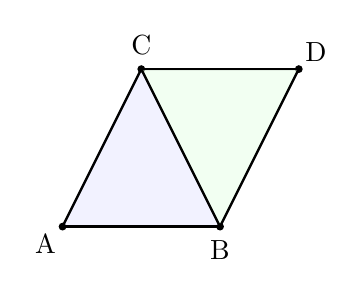
\begin{tikzpicture}[scale=2, thick, every node/.style={circle, inner sep=1pt, fill=black}]
  % Nodes
  \node (A) at (0,0) [label=below left:A]{};
  \node (B) at (1,0) [label=below:B]{};
  \node (C) at (0.5,1) [label=above:C]{};
  \node (D) at (1.5,1) [label=above right:D]{};

  % Triangle ABC
  \draw[fill=blue!10, opacity=0.5] (A.center) -- (B.center) -- (C.center) -- cycle;
  % Triangle CBD
  \draw[fill=green!10, opacity=0.5] (B.center) -- (C.center) -- (D.center) -- cycle;

  % Edges
  \draw (A.center) -- (B.center);
  \draw (B.center) -- (C.center);
  \draw (C.center) -- (A.center);
  \draw (C.center) -- (D.center);
  \draw (B.center) -- (D.center);
\end{tikzpicture}
\end{center}

\subsection*{Interpretation}

In this example:
\begin{itemize}
  \item The triangles \(\triangle ABC\) and \(\triangle CBD\) are both elements of \(X_2\).
  \item The edge \(BC\) is a common face of both.
  \item This gluing is encoded purely via face maps in the functor \(X : \Delta^{\text{op}} \to \mathbf{Set}\), not through geometric topology.
\end{itemize}

Thus, \(\mathbf{SSet}\) encodes how simplices are assembled by tracking how their faces are identified via morphisms in \(\Delta\).




\subsection*{Definition: Kan Complex and the Kan Condition}

Let \(X\) be a simplicial set.

For each \(n \geq 1\) and \(0 \leq k \leq n\), the **\(k\)-th horn** \(\Lambda^k[n]\) is the sub-simplicial set of \(\Delta[n]\) (the standard \(n\)-simplex) consisting of all \((n-1)\)-faces except the \(k\)-th one.

A **Kan filler** is a map:
\[
\Lambda^k[n] \to X \quad \text{that extends to} \quad \Delta[n] \to X
\]

\paragraph{Kan Condition.}
A simplicial set \(X\) is a **Kan complex** if for every such horn map \(f : \Lambda^k[n] \to X\), there exists a map \(\tilde{f} : \Delta[n] \to X\) making the diagram commute:
\[
\begin{tikzcd}
\Lambda^k[n] \arrow[r, "f"] \arrow[d, hook] & X \\
\Delta[n] \arrow[ru, dashed, "\tilde{f}"'] &
\end{tikzcd}
\]

\paragraph{Interpretation.}
This means: whenever you specify all but one face of an \(n\)-simplex in \(X\), you can find a full simplex in \(X\) that completes it.

\paragraph{Why It Matters.}
\begin{itemize}
  \item It allows definition of **paths** between 0-simplices (vertices)
  \item And **homotopies** between such paths (using 2-simplices)
  \item And so on, inductively, for all higher dimensions
\end{itemize}

Thus, **Kan complexes are combinatorial models of homotopy types.**


\subsection*{Identity Types in Homotopy Type Theory (HoTT)}

In Martin-Löf Type Theory, the identity type \(\mathrm{Id}_A(a, b)\) expresses that two terms \(a, b : A\) are equal.

In Homotopy Type Theory, this is reinterpreted:
\[
\mathrm{Id}_A(a, b) \quad \text{is the type of paths from } a \text{ to } b \text{ in the space } A
\]

\paragraph{Simplicial Model.}
Let \(X \in \mathbf{SSet}\) be a Kan complex.

\begin{itemize}
  \item \(X_0\): 0-simplices = points (terms of type \(A\))
  \item \(X_1\): 1-simplices = edges (proofs of identity)
\end{itemize}

A 1-simplex \(\alpha \in X_1\) represents a path from \(a\) to \(b\) if:
\[
d_1(\alpha) = a, \quad d_0(\alpha) = b
\]

This realizes \(\alpha : \mathrm{Id}_A(a, b)\) in the type-theoretic sense.

\paragraph{Higher Identity Types.}
\begin{itemize}
  \item 2-simplices in \(X\): homotopies between identity proofs (paths between paths)
  \item 3-simplices: coherence between homotopies
  \item etc.
\end{itemize}

The full tower of identity types is modeled using higher simplices.

\paragraph{Kan Condition Enables This.}
The Kan filler condition ensures that:
\begin{itemize}
  \item Paths can always be completed
  \item Homotopies can always be constructed between composable paths
  \item Higher coherence structures exist as needed
\end{itemize}

Thus, a Kan complex faithfully models the identity structure of a type in HoTT.







\section{From Static HoTT to Dynamic HoTT: A Philosophical and Logical Cartography}

The topological concepts we've just explored—spaces, paths, and homotopies—are not mere mathematical curiosities. They form the very language Homotopy Type Theory (HoTT) uses to rethink fundamental logical notions like types, terms, and identity. This section bridges these mathematical ideas to the core argument of our book: the need to move from a static understanding of these structures to a dynamic one.

HoTT offers a profound connection between type theory (a formal system from logic and computer science) and homotopy theory (a branch of topology). In HoTT:
\begin{itemize}
    \item \textbf{Types are interpreted as spaces} (specifically, as $\infty$-groupoids or homotopy types). The abstract notion of a 'type' (like 'the type of animals' or 'the type of numbers') is given a geometric interpretation as a space.
    \item \textbf{Terms of a type are interpreted as points} in the corresponding space. An individual animal or a specific number would be a point in its respective type-space.
    \item \textbf{Identity types (equality) are interpreted as path spaces.} An element $p: (a =_A b)$ of the identity type, witnessing that terms $a,b:A$ are equal, is interpreted as a path (as in Definition \ref{def:path}) from point $a$ to point $b$ in the space $A$. So, equality isn't just a binary relation; it's a structured object—a path.
    \item \textbf{Higher identity types correspond to higher path spaces (homotopies).} An equality between two proofs of equality $p, q: (a =_A b)$ is a path between the paths $p$ and $q$ (a 2-path, or homotopy, as in Definition \ref{def:homotopy}). This hierarchy extends infinitely, mirroring the structure of an $\infty$-groupoid (Definition \ref{def:higher-paths}).
\end{itemize}

Traditional HoTT, as often presented, implicitly treats these type-spaces as stable, static universes of mathematical objects. The richness comes from the internal homotopical complexity of these static universes. However, many philosophical questions about meaning, consciousness, and language involve change, context-dependence, and evolution—dynamics that a static picture struggles to capture. Dynamic Homotopy Type Theory (DHoTT), the subject of this book, extends this foundation by introducing an explicit notion of \emph{change} or \emph{evolution} of these semantic spaces themselves, often indexed by a temporal or contextual parameter (which we might denote abstractly as $\tau$). In DHoTT, types (semantic spaces) can transform, reconfigure, or even undergo "ruptures" as contexts shift, leading to a dynamic landscape where meaning itself is subject to drift and re-formation.

\subsection{Static HoTT: A Brief Recap of Core Ideas}

In standard HoTT, the foundational correspondences are:
\begin{itemize}
  \item \textbf{Types as spaces}: A type $A$ is understood as a topological space $|A|$ (more precisely, its homotopy type or $\infty$-groupoid). The abstract concept of a "type" is given a geometric meaning.
  \item \textbf{Terms as points}: An element $a:A$ corresponds to a point in the space $|A|$. A specific instance of a type is a location in this space.
  \item \textbf{Identity as paths}: An identification or equality $p: (a =_A b)$ between terms $a, b : A$ is represented by a continuous path in $|A|$ connecting the point corresponding to $a$ to the point corresponding to $b$. The type $a =_A b$ is itself a type (a space of paths). This means "being equal" can have structure.
  \item \textbf{Higher identities as homotopies}: Equalities between paths (identifications $q: (p_1 =_{ (a=_A b) } p_2)$) correspond to homotopies between these paths (2-paths). This continues, forming the $\infty$-groupoid structure inherent in each type. This allows for reasoning about different ways equalities can themselves be equal.
\end{itemize}
A key principle is \textbf{univalence}, which states that type isomorphism $A \simeq B$ (two types having the same structure) is equivalent to identity $A = B$ (the types themselves being equal).

\subsection{Canonical Representation and Notation (HoTT vs. DHoTT Glimpse)}

In canonical HoTT texts (e.g., "Homotopy Type Theory: Univalent Foundations for Mathematics," also known as The HoTT Book):
\begin{itemize}
  \item Identity types are often written as $x =_A y$ or $\operatorname{Id}_A(x,y)$.
  \item Dependent product types (forming functions) are written as $\Pi_{x:A} B(x)$ or $(x:A) \to B(x)$.
  \item Dependent sum types (forming pairs) are written as $\Sigma_{x:A} B(x)$ or $(x:A) \times B(x)$.
  \item Equivalences between types (isomorphisms in the homotopical sense) are denoted $A \simeq B$.
\end{itemize}

In DHoTT, we will build upon this foundation. While many notations remain similar, new constructs will be introduced to handle dynamics. Philosophically, this is where we begin to address how meaning isn't fixed but evolves:
\begin{itemize}
  \item Identity paths remain crucial: $x =_A y$.
  \item The notion of a type $A$ \emph{drifting} or transforming into another type $A^{\dagger}$ due to a contextual shift $\tau$ might be indicated by notations like $A \stackrel{\tau}{\rightsquigarrow} A^{\dagger}$ or through indexed types $A(\tau)$. This directly addresses the philosophical concern that the meaning of concepts (types) can change over time or with context.
  \item The coherence of terms and structures under such drifts will be a central concern, potentially involving constructs like $\mathcal{R}^\star_\tau(a)$ to denote the trace or evolution of a term $a$ under drift $\tau$. This tackles how an individual meaning (term) maintains its identity or transforms as its conceptual category (type) evolves.
\end{itemize}
These DHoTT-specific notations will be formally introduced and developed in the subsequent chapters. This preliminary chapter aims to provide the classical mathematical and HoTT backdrop against which these dynamic extensions, motivated by the fluid nature of meaning and consciousness, will be defined.
